\documentclass[oneside]{nccuthesis}
\usepackage{times}
\usepackage{verbatim}
\usepackage{color}
\usepackage{url}
\usepackage{graphicx}
\usepackage{array}
\usepackage{pdfpages} % include outside .pdf
\usepackage{wallpaper} % watermark
% for table generate
\usepackage{mathtools}
\usepackage{amsmath}
\usepackage{amssymb}
\usepackage{booktabs}
\usepackage{adjustbox}
\usepackage{longtable}
\usepackage{multirow}
% Format the refs
%\usepackage[sort,comma,square ]{natbib}
\usepackage[hidelinks]{hyperref}
% For the tree
\usepackage{tikz}
\usepackage{tikz-qtree}

%Bibliography style
\bibliographystyle{acm}

% For barchart
\usepackage{pgfplots}

% Using the tex-text mapping for ligatures etc.
\defaultfontfeatures{Mapping=tex-text}

% Set the default fonts
\setmainfont{Times New Roman}
\setCJKmainfont{AR PL UKai TW}
\setCJKmonofont{AR PL UKai TW}

% Your information goes here
% author: Tz-Huan Huang [http://www.csie.ntu.edu.tw/~tzhuan]

% ----------------------------------------------------------------------------
% "THE CHOCOLATE-WARE LICENSE":
% Tz-Huan Huang wrote this file. As long as you retain this notice you
% can do whatever you want with this stuff. If we meet some day, and you think
% this stuff is worth it, you can buy me a chocolate in return Tz-Huan Huang
% ----------------------------------------------------------------------------

% Syntax: \var{English}{Chinese}
\university{National Chengchi University (NCCU)}{國立政治大學}
\college{College of Science}{理學院}
\institute{Department of Computer Science}{資訊科學系}
\title{Portfolio Management System with Risk Preference Adjusted Utility Function}
{具風險偏好調整效用函數之資產配置系統}
\author{Tain-Tzu Chang}{張天慈}
\studentid{108971001}
\advisor{Yuh Jong Hu, Ph.D.}{胡毓忠\ 博士}
\defenseyear{2021}{一一零}
\defensemonth{July}{七}
\defenseday{17}

\pgfplotsset{compat=1.14}
\begin{document}

% 政大論文浮水印

\input{src/with-watermark.tex}

\hypersetup{pageanchor=false}

\frontmatter
\pagenumbering{gobble}
\makecover

\clearpages
\setcounter{page}{1}
\hypersetup{pageanchor=true}
\pagenumbering{roman}
\phantomsection
\ClearWallPaper
% generate certification
% \makecertification
% or include scanned pdf
%\addcontentsline{toc}{chapter}{口試委員會審定書}
%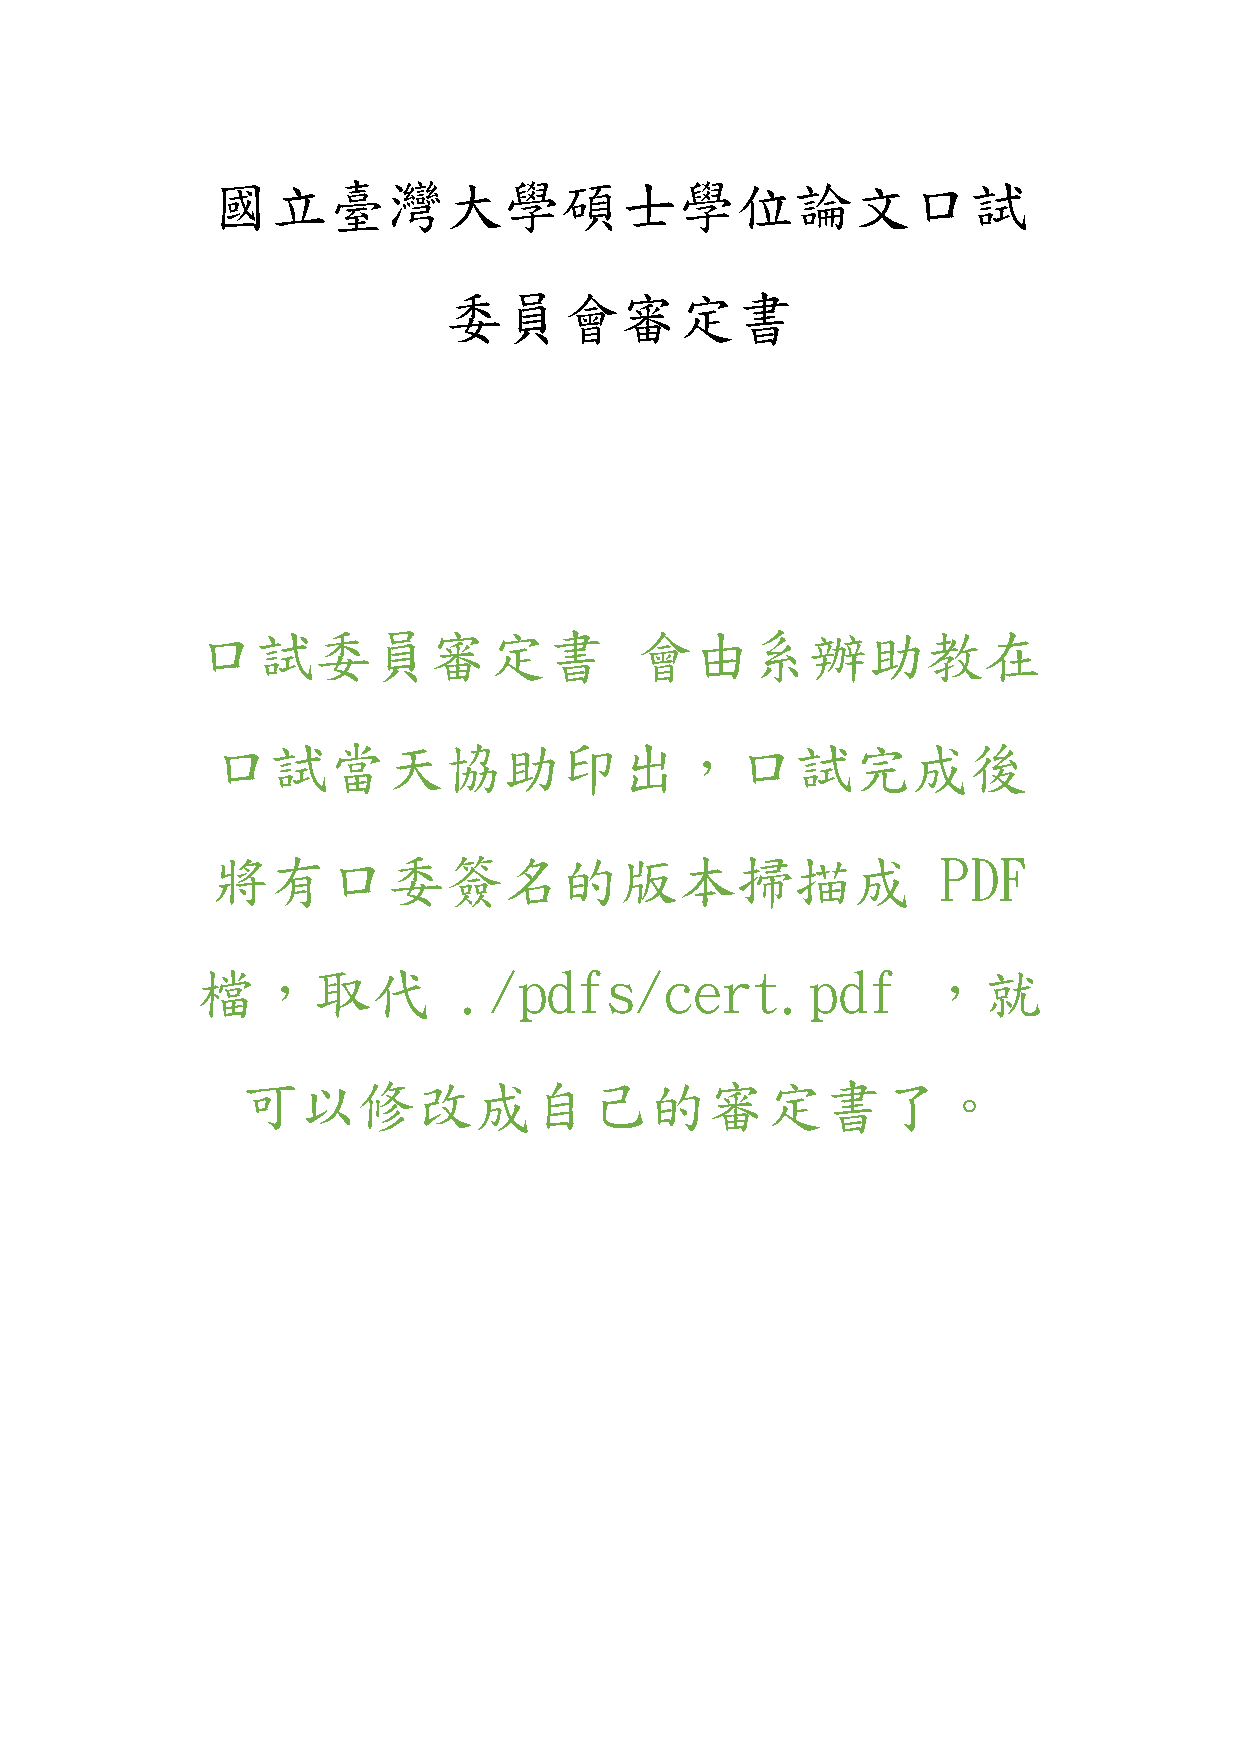
\includepdf[pages={1}]{pdfs/cert.pdf}


\begin{acknowledgementszh}
這是中文行距測試,應該看到一點五倍行距。這是中文行距測試,應該看到一點
五倍行距。這是中文行距測試,應該看到一點五倍行距。這是中文行距測試,應
該看到一點五倍行距。這是中文行距測試,應該看到一點五倍行距。這是中文行
距測試,應該看到一點五倍行距。這是中文行距測試,應該看到一點五倍行距。
這是中文行距測試,應該看到一點五倍行距。這是中文行距測試,應該看到一點
五倍行距。這是中文行距測試,應該看到一點五倍行距。這是中文行距測試,應
該看到一點五倍行距。這是中文行距測試,應該看到一點五倍行距。這是中文行
距測試,應該看到一點五倍行距。這是中文行距測試,應該看到一點五倍行距。

感謝\ldots
\end{acknowledgementszh}

\begin{acknowledgementsen}


I'm glad to thank\ldots 
\end{acknowledgementsen}

\begin{abstracten}
Requirements for portfolio management is different among different investors. Risk is one of the critical factors. Max Drawdown (MDD), the maximum observed loss from a peak to a trough of a portfolio, is a commonly used risk indicator. Reinforcement Learning (RL) is a promising machine learning approach for portfolio selection. Instead of using investment return as a reward function directly, many models use indicators that have taken variability into account, like Sharpe Ratio \cite{Sharpe49} or Sterling ratio. However, neither Sharpe ratio nor Sterling ratio has inputs to raise or reduce risk's influence upon the reward function. Therefore the model using Sharpe Ratio \cite{Sharpe49} or Sterling ratio cannot reflect the needs of investor types with different tolerance to risk.

\par
In this thesis, we introduce a reward function for Portfolio Management RL model which includes the influence of MDD as its parameters.   

asset allocation reinforcement learning reward function


\noindent
Keywords: Reinforcement Learning, Max Drawdown, Portfolio Management,
\end{abstracten}


% Table of Content
\clearpages
\tableofcontents
% List of Figures
\clearpages
\listoffigures
% List of Tables
\clearpages
%\listoftables

\mainmatter

% Your thesis goes here
% \chapter{Introduction}
\section {Background}
A portfolio is a collection of financial investments. The goal of portfolio selection is to construct an optimal portfolio, which is usually different between investors due to their characteristics. Among these characteristics, risk preference is one of the significant factors. There are many indicators to represent the risk of the portfolio. Maximum Drawdown (MDD),  maximum loss from a peak over a given period, is a commonly used indicator of the risk.

Traditionally portfolio selection can be divided into two stages. Frist stage constructs the belief of future performance of available financial products. The second stage starts from the first stage and produces the choice of portfolio.  Modern Portfolio Theory (MPT) introduced by  Harry Markowitz \cite{10.2307/2975974} focus on the second stage. Machine Learning (ML) or Reinforcement Learning (RL) can complete both stages in a single process and construct portfolios that out-performed the general market.\cite{KRAUSS2017689}
\section {Motivation}
Psychologically, humans favor avoiding losses to acquire equivalent gains. This tendency is called Loss Aversion.\cite{kahneman2000analysis} Kahneman's study suggests losses are twice as powerful as gains.\cite{Tversky1992} With Modern Portfolio Theory (MPT), we can construct a portfolio that produces the maximum expected return from a given variance, an indicator of risk, or vice versa, the minimal variance from a given expected return.\cite{10.2307/2975974} MPT can construct portfolios fits different investors' preference.
Although many portfolio performance measures are risk-adjusted\cite{cogneau2009101,cogneau2009more,cogneau2009more2}, like the Shape ratio\cite{Sharpe49} or the Sterling ratio\cite{magdon2004maximum}, most of them do not incorporate investors' risk preferences. Constructing portfolios based on investors' risk preferences will challenge machine learning models optimizing with these measures.

\section {Research Objective}
This thesis aims to introduce an objective function and incorporate conventional Deep Reinforcement Learning (DRL) models to construct portfolios that fit investors with different risk preferences. The expected Maximum Drawdown (MDD) of the portfolio will represent investors' risk preferences and adjust the portfolio performance measure, which will be the objective function incorporate with DRL models to construct portfolios based on investors' risk preferences.
\label{c:intro}


% \chapter{Related Work}
\label{c:related}

%\section{First}
%\label{s:related1}

\section{Risk Adjusted Measures of Performance}
There are many portfolio performance measures.\cite{cogneau2009101,cogneau2009more,cogneau2009more2}
Risk-Adjusted measures incorporate risk into the measure of performance for finance investments and reflect investors' nature better than using return along.
We will discuss a few of them over here.
\subsection{Sharpe Ratio}
Sharpe Ratio\cite{Sharpe49} is one of the most well-known risk-adjusted measure. It represent amount of return per unit of variation, or risk.\\
The revision version is defined as
\[ SR = \frac{E(R_a - R_b)}{\sigma_a},
\sigma_a = \sqrt{VAR(R_a-R_b)}\]
where \(R_a\) is the return of the assert, 
\(R_b\) is the risk-free return,
\(E(R_a - R_b)\) is the expected excess return of the assert,
and \(\sigma_a\) is standard deviation of the excess return.
One downside of the Sharpe Ratio is that it penalizes occasional high returns\cite{9206647}.
\subsection{Sterling ratio}
Sterling ratio\cite{magdon2004maximum} uses max drawdown (MDD) over a given period to represent the risk; this resolves the issue Sharpe Ratio has with occasional high returns. 
There are many forms of Sterling ratio; one common definition\cite{magdon2004maximum} is defined as 
\[ SR = \frac{E(R_a - R_b)}{MDD - 10\%}\]
\subsection{Calmar ratio}
Calmar ratio\cite{young1991calmar} replace empirical max drawdown with the expected maximum drawdown \(E(MDD)\), defined as 
\[C_T = \frac{E(R_a - R_b)}{E(MDD)}\]


\subsection{Other Measures of Performance}
There are many other Sharpe ratio variations, like Burke Ratio, Martin Ratio, or Pain Ratio\cite{bacon2009sharp}. Furthermore, Philippe Cogneau and Georges Hübner censused the 101 performance measures for portfolios. Many of the measures are risk-adjusted measures\cite{cogneau2009101,cogneau2009more,cogneau2009more2}.
\section{Modern Portfolio Theory (MPT)}
Harry Markowitz introduced modern portfolio theory (MPT) in 1952. Instead of maximizing the expected return, the objective of MPT is to find the maximum expected return on a given risk. The variance of the portfolio is used as an indicator of risk. \cite{10.2307/2975974}
\par
For an N assets portfolio, \(E(R_i)\) and  \(\sigma_i\) is the expected return and standard deviation of the asset \(i\). \(w_i\) is the weighting of the asset in the portfolio.\(\rho_{ij}\) is the correlation coefficient between the returns on assets i and j.
The expected return and variance of the portfolio, \(E(R_p)\) and \(\sigma_p^2\), are defined as:
\[E(R_p) = \sum_i^N w_i E_i\]
\[\sigma_p^2 = \sum_i \sum_j w_i w_j \sigma_i \sigma_j \rho_{ij}\]
where
\[\forall w: w \geq 0 \quad \sum_i ^N w_i = 1\]
\par
The next step is plot expected return and variance of all portfolios and find the efficient frontier. Than we can identify the portfolio with the maximize return on a given risk, or, vice versa, the lowest risk on a given expected return from the efficient frontier.
\section{Financial Market Predictions with Machine Learning}
Machine Learning has become a powerful tool in many fields, including finance. Christopher Krauss successfully used various machine learning techniques, including deep neural networks, gradient-boosted-trees, and random forests, to create ensembles predicting the S\&P 500 index that out-performed the general market\cite{KRAUSS2017689}.
\par

Thomas Fischer brings deep learning to the next level by using Long Short-Term Memory (LSTM) network\cite{FISCHER2018654}. His model demonstrates LSTM can effectively extract meaningful information from noisy financial time series data and beat other machine learning models in  Christopher Krauss's article  \cite{KRAUSS2017689} for most situations, except the crisis in 2009, where Random Forest perform better than LSTM.
\section{Trading systems with Reinforcement Learning}
John Moody and Lizhong Wu introduced Reinforcement Learning for the trading system \cite{618952}. Trading systems trained via Reinforcement learning can incorporate the effects of transaction costs and taxes. The result of such systems outperformed trading systems trained via supervised learning with labels. For objective function, they observed maximizing the differential Sharpe ratio yields more consistent results than maximizing profits\cite{618952,moody1998performance}.\\
The differential Sharpe ratio \(D\) is defined as:
\[
\cfrac{d D_t}{d R_t} = 
\cfrac{B_{t-1}-A_{t-1} R_t}{(B_{t-1}-A_{t-1}^2)^\frac{3}{2}}
\]
where
A and B is the first and second moments of the returns' distributions
\[ A_n = \cfrac{1}{n}\sum_{i=1}^nR_i\quad
B_n = \cfrac{1}{n}\sum_{i=1}^nR_i^2
\]

Saud Almahdi uses a coherent downside risk measure, the Calmar ratio,  as the objective function for Reinforcement Learning \cite{AdaptivePortfolioTradingSystem}. They show that the portfolios constructed using RRL with the expected maximum drawdown based Calmar ratio results yield better performance and transaction cost resilient than the portfolios constructed with the Sharpe ratio. 






\cite{AdaptivePortfolioTradingSystem}
\section{Soft Actor-Critic (SAC)}
Soft Actor-Critic (SAC)\cite{haarnoja2018soft}


% \chapter{Reinforcement Learning}
\section{Overview}
Reinforcement Learning (RL) is a machine learning technique that simulates an agent interacting with the environment. Typical scenario:
    \begin{enumerate}
        \item The agent observes the states from the environment.
        \item The agent performs the action on the environment based on the state observed.
        \item The environment feedback rewards to the agent based on the action performed; the agent will adjust its behavior based on the reward. 
    \end{enumerate}
\begin{figure}[ht]
  \centering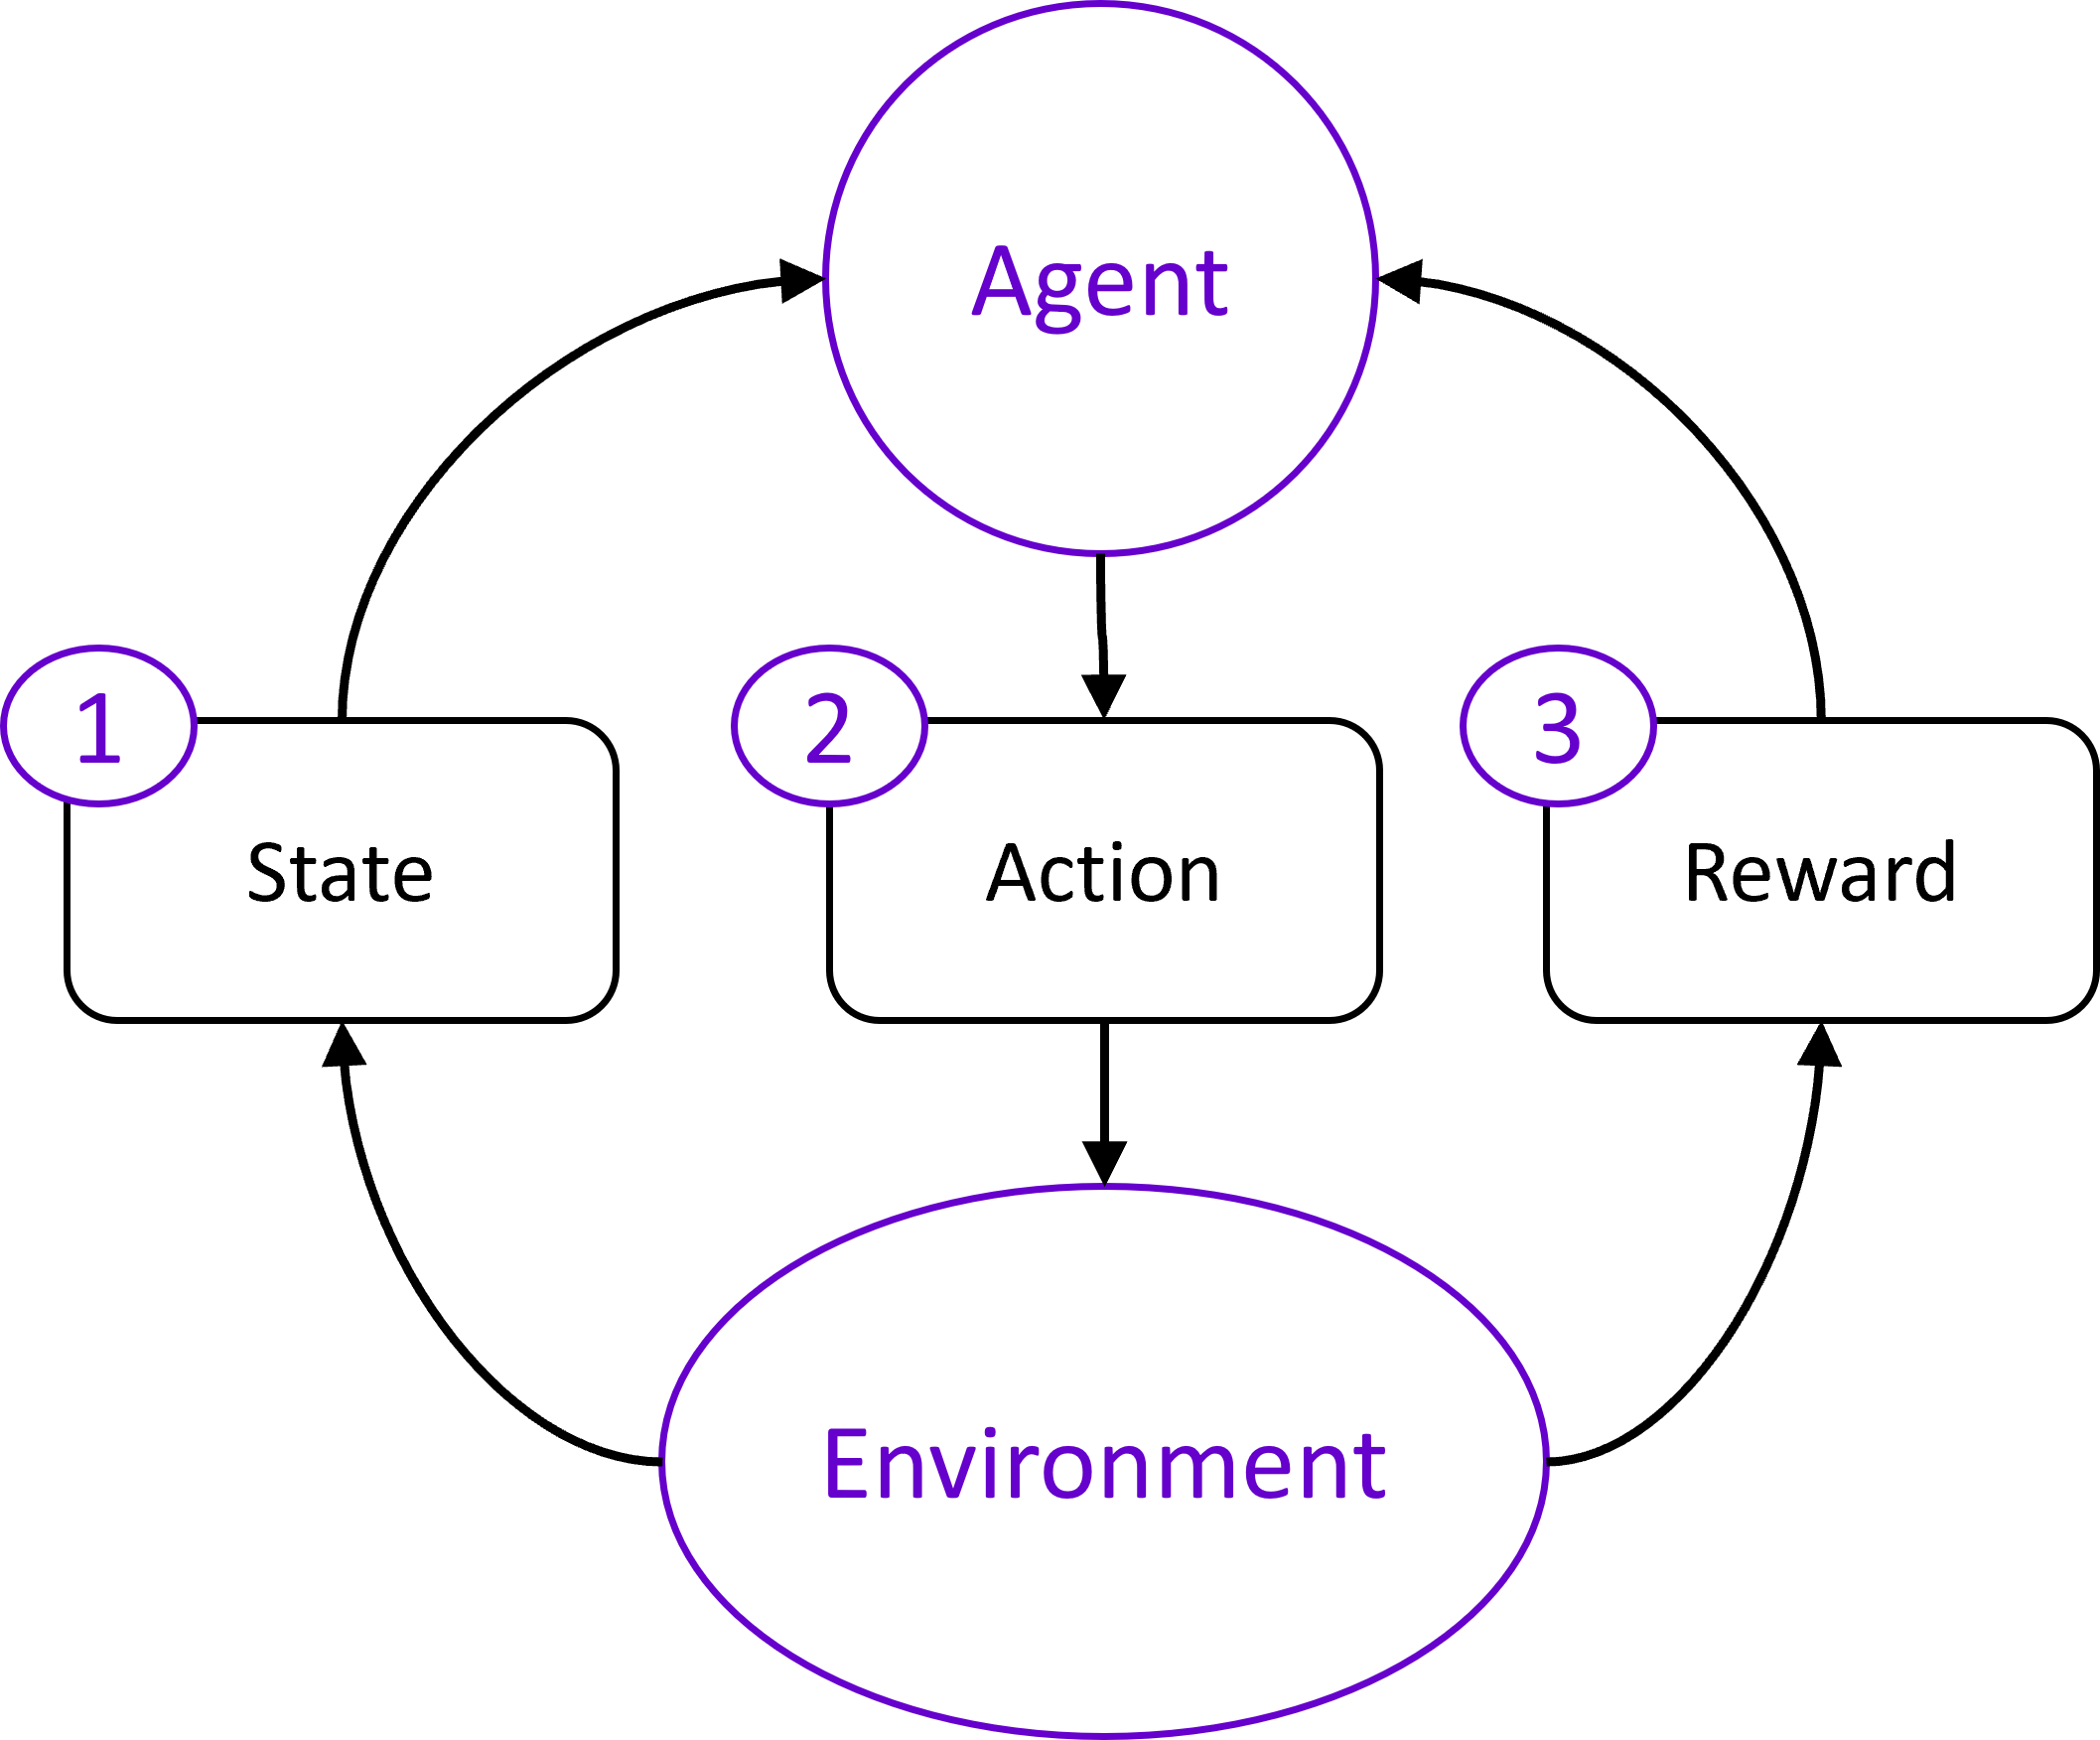
\includegraphics[width=8cm]{images/rl_overview.png}
  \caption [Overview of Reinforcement Learning]
  {Overview of Reinforcement Learning
  }
  \label{fig:rl_overview_diagram}
\end{figure}

\section{Value Function}
The value function is the function to predict the expected reward based on given states and actions. The off-policy algorithm uses value function, e.g., Q learning will have a high sample efficiency with the use of experience replay but will face significant challenges for continuous action spaces since the output space of the value function will be enormous.
\section{Policy}
The policy is the strategy of the agent to perform the action that maximizes the expected reward based on the state.  The typical algorithm uses policy, Policy Gradient can work well with high dimension or continue action spaces. But it has low sample efficiency as it requires a full episode before adjusting the parameters.
\section{Actor Critic}
Actor-Critic uses both the Value Function and the Policy. The actor determines the actions with the policy. The critic uses the value function to criticize the actor's action. Actor-Critic can have high sample efficiency with continuous action spaces.

\section{Deep Reinforcement Learning}
Deep Reinforcement Learning (DRL) combines reinforcement learning (RL) and deep learning. DRL archive remarkable results in many fields, including gaming. We can adapt deep learning networks in many different components of RL, including the value function, or the policy.
\section{Soft Actor-Critic}
Soft Actor-Critic (SAC) is an DRL algorithm that optimizes a stochastic policy in an off-policy way with entropy regularization.
\par
Compare to deterministic policies, stochastic policies provide a stabler result as it favor exploration.
\par 
As a off-policy algorithm, SAC have better sample efficiency with experience replay.
\par
Entropy Regularization balances the exploration-exploitation trade-off as the algorithm favors exploration when the entropy is high initially and becomes more deterministic when entropy is low to increase exploitation.
% \chapter{System Design}
\label{c:system_design}
\section{Overview}
\autoref{fig:context_diagram} represents the overview and workflow of our proposed DRL-based Portfolio Management System.
The system will output portfolios based on the inputs, the market the investment universe, and investor preference. 
\par
The system contains two main parts, the DRL model and the trading environment. We will detail discuss about them in \autoref{c:drl} and \autoref{c:trading_environment}. The trading environment bridges domain-specific inputs/outputs with the general-purpose DRL model. This architecture enables the system to function with most existing DRL models with ease. 
 
\begin{figure}[hbt]
  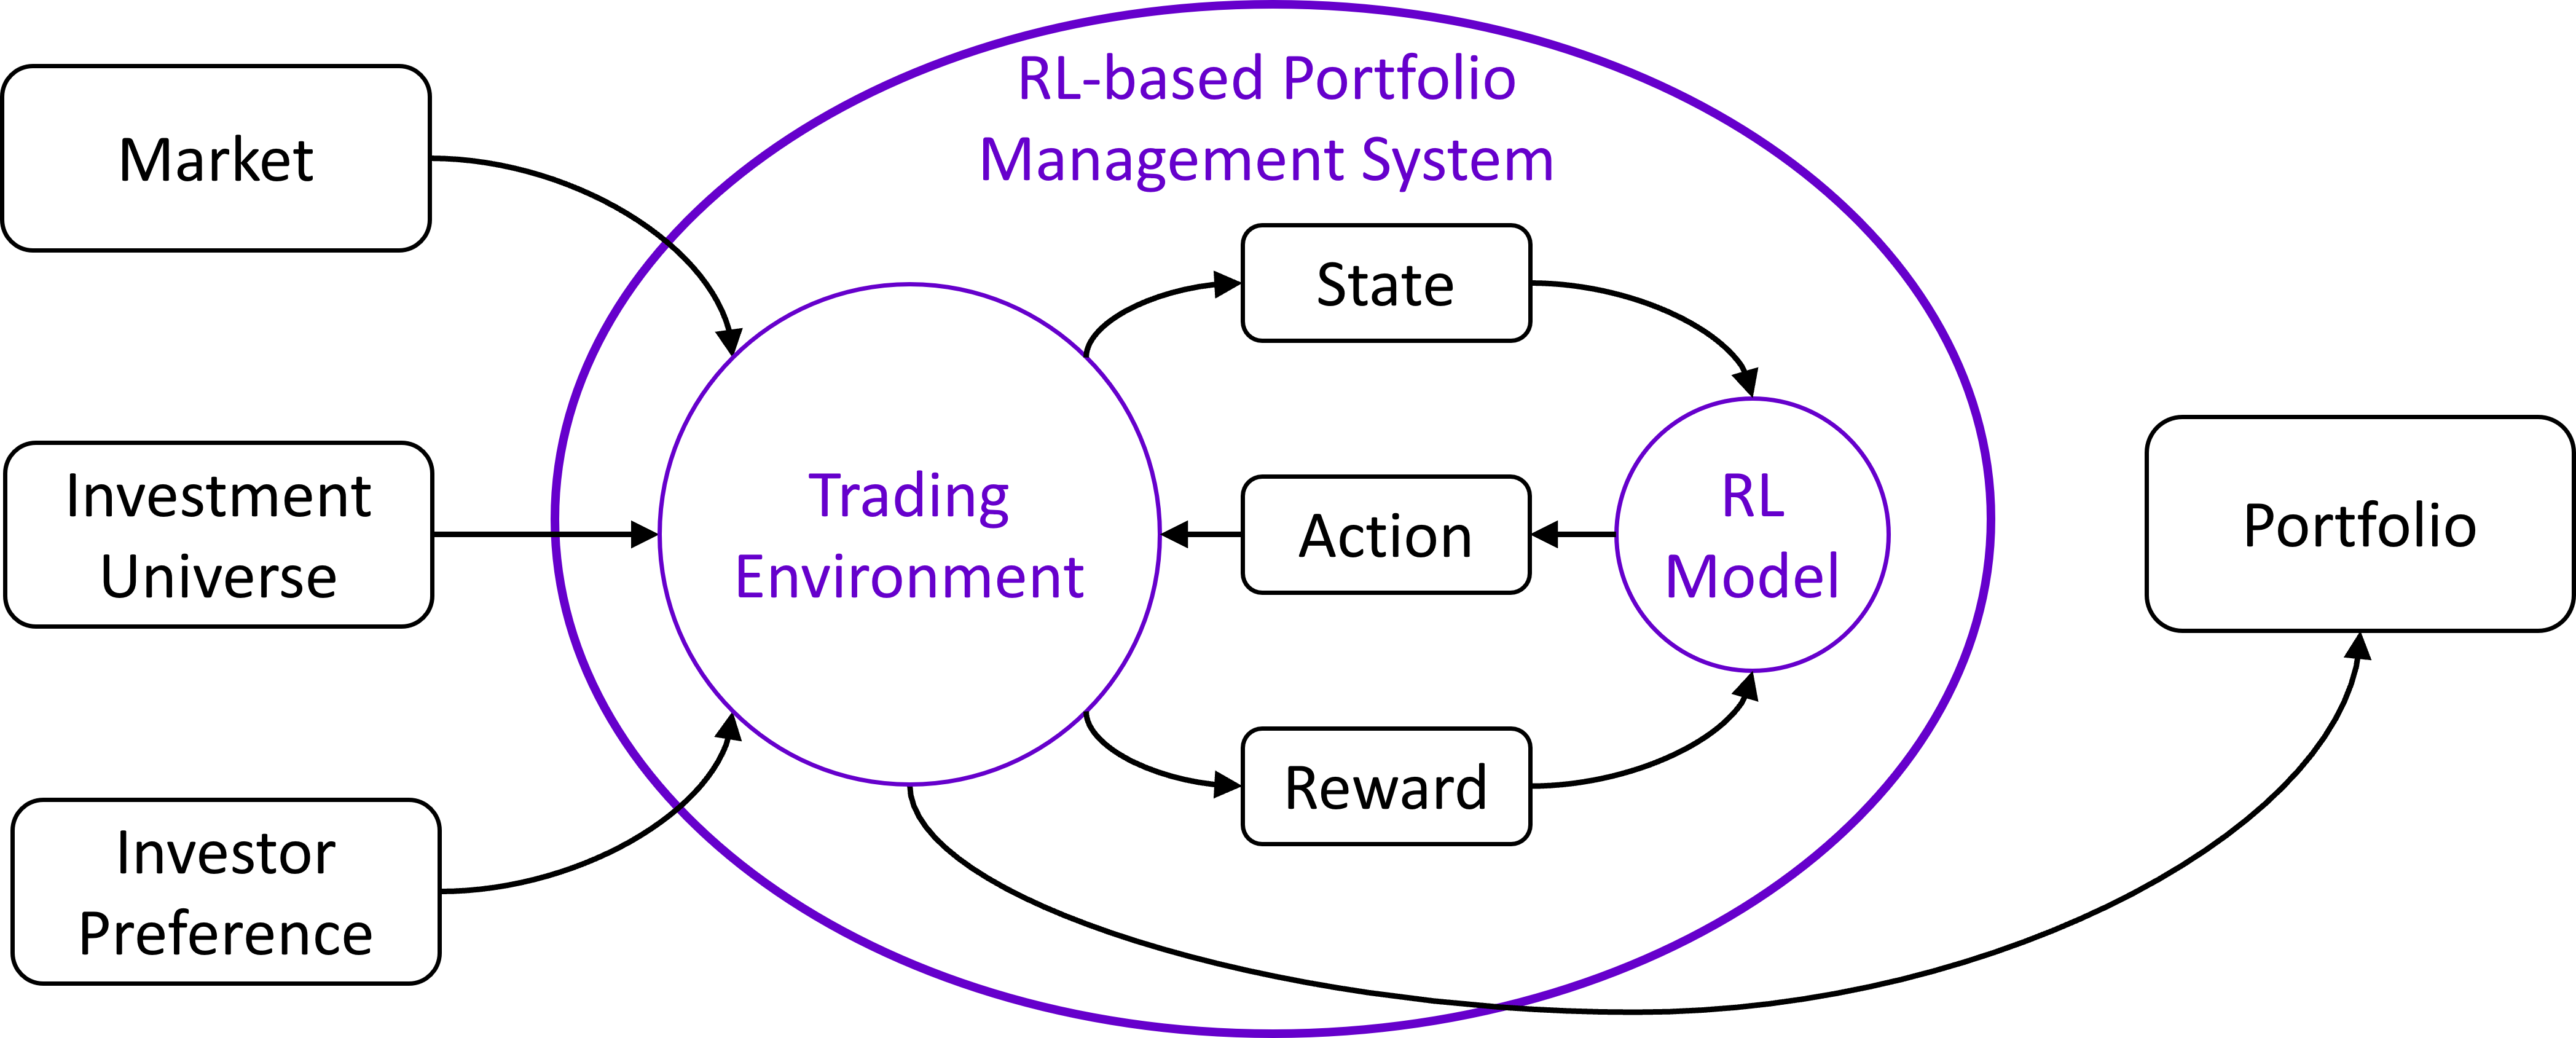
\includegraphics[width=15cm]{images/context_diagram.png}
  \caption{Context Diagram}
  \label{fig:context_diagram}
\end{figure}
\section{Investment Universe}
The investment universe is a collection of investable investments for the portfolio management system. The goal is to choose investments with low covariances between each other; hence their combinations can yield better profits from the same risk level\cite{willenbrock2011diversification}. 
\par 
Meir Statman suggested that a well-defined portfolio should have at least 30 or 40 stocks,  \cite{statman1987many}. However, most Exchange Traded Funds (ETFs) combine many investment products and offer investor diversification. Least than ten ETFs are sufficient to produce portfolios with adequate diversification \cite{chang_2016}.
\par
We start from the top 100 ETFs by Asset Under Management (AUM) on March 2021 and remove ones with trading records of less than 14 years. We then obtain the top two most correlated ETFs and remove the one with lower AUM and continue the same process iteratively until 10 ETFs are left (\autoref{appendix:etfs_corr}).
\par
Our selection shows a wide diversity in return and risk, represented in CAGR and stand division of returns. 
\begin{figure}[bth]
    \centering
    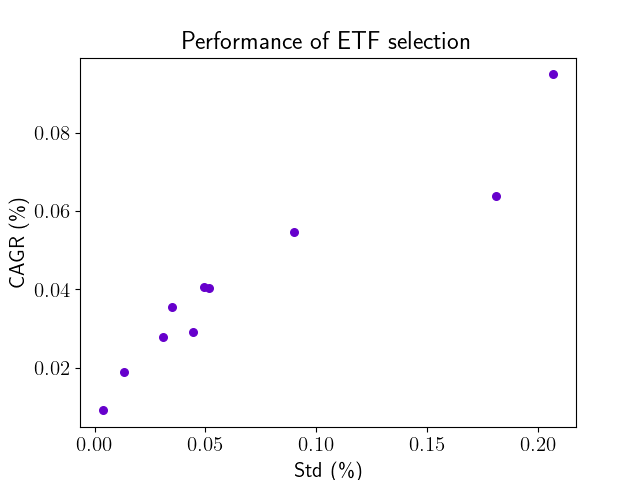
\includegraphics[width=12cm]{images/etfs.png}
    \caption{Performance of ETFs}
    \label{fig:efts}
\end{figure}
\section{Market Features}
The model uses structured information from the market as its data source, including interest rates, commodity prices and currency exchange indexes. (\autoref{appendix:features_list}).
\par
For stationary data, we will use them directly as features. For non-stationary data, we use statistics measures among 5, 20, and 60 days as features, including standard deviation, skewness, and kurtosis.
\par
Features are collected and calculated beforehand and stored in files for further usage. They will be used as part of the inputs to construct the trading environment used for training and validation.
\section{Investor Preference}
For investor preference, we will focus on the risk preference of the investors. Usually, professional personnel or organization will acquire risk preference from investors by survey or other techniques and interprets the inputs into comparable risk measure indicators between investors. 
\subsubsection{Standard Deviation}
We can measure the volatility of the return with the standard deviation. The well known Sharpe Ratio uses the standard deviation to represent a risk. The downside for the standard deviation of return is assets that produce a blooming return that most investors seek will also yield a high standard deviation.
\subsubsection{Maximum Drawdown}
Drawdown is the decline from the highest peak. Maximum drawdown (MDD) is the maximum decline over the given period and reflects the actual loss of the investors. We use MDD as be one of the indicators to evaluate our system. 
\par
However, optimizing any ratio using MDD directly has many problems and challenges. Some researches indicate MDDs are outliers \cite {johansen2002large, johansen1998stock} or imply optimizing MDD is troublesome \cite{moody1998performance}. Therefore, we will not limit ourselves to use MDD while optimizing the model and consider other alternatives. 
\section{Deep Reinforcement Learning Model}
As our action spaces are continuous, we will not use Value function-based DRL algorithms, e.g., DQN, since the output stage will be enormous. We have limited sample data since we will use real-world data, not data from a simulation environment. We will rule out on-policy algorithms as it is beneficial to use an experience replay set to utilize the sample efficiently.
\par
Based on the requirements above, we have DDPG, TD3, and SAC as our candidates. We use SAC as our DRL model since it optimizes a stochastic policy with entropy regularization, reducing the chances of the system trapped in local optimal and balance the exploration-exploitation dilemma.

We used SAC \cite{haarnoja2018soft} provided in RLkit, an open-source RL framework implemented in PyTorch\cite{pongrlkit}, as our RL model.
\

\chapter{Methodology}
\section{Dataset}
\subsection{Data Collection}
We collected the historical adjusted closed prices of EFTs (\autoref{appendix:etfs_corr}) and market features (\autoref{appendix:features_list}) between 2007/4/20 til  2021/3/15 from Yahoo Finance and Federal Reserve Economic Data. We use data before 2017/2/28 as the training data and the rest as validation data.
\begin{table}[ht]
    \centering
        \begin{tabular}{|c|c|c|c|}
        \hline \hline
        Data Type & Start Time & End Time & Period (Year) \\ \hline
        Training Data  &  2007/4/20 & 2017/2/28 & 9.87\\ \hline
        Validation Data & 2017/3/1 & 2021/3/15 & 4.04 \\ 
        \hline \hline
        \end{tabular}
    \caption{Data Collection Period}
    \label{tab:dataset}
\end{table}


\subsection{Data Processing}
The data we collected are structured data; we only need to fill the missing data with the nearest pass data and calculate statistics measures for non-stationary data.  All data processed are stored in files for further usage to improve efficiency. 
\section{Holding and Transaction Costs}
The extra costs which we did not take into account are the holding costs and the transaction costs.
\par
The holding costs are the expenses paid to the ETF issuer for administration and operation. For most holding costs, ETFs are trivial; for example, SPY has a  gross expense ratio least than 0.1\%, and it is not the lowest among other ETFs. We assume holding costs is inconsequential to our result.
\par
The transaction costs are the costs during the transaction, including commission. Many ETFs are commission-free; we assume the transaction costs will not significantly impact our experiment result if we trade infrequently.
\section {Hyper Parameter}
As the default hyperparameters of SAC, except reward scale, produces good results on various environments in the original paper\cite{haarnoja2018soft}.  
We only adjusted the reward scale and kept the rest as default.
\par
SAC is highly sensitive to the scaling of the reward. If the reward scale is too small, the reward will fail to affect the model, and the policy will become nearly uniform. The model will learn quickly and become deterministic for the reward scale too large, leaving no room for exploration.
\par
\begin{table}[htb]
    \centering
    \begin{tabular}{| c|c | }
   \hline \hline
   Parameter & Value \\ \hline \hline
   Optimizer & Adam \\ \hline
   Learning rate & \(3 10^{-4}\) \\ \hline
   Replay size & \(10^6\) \\ \hline
   Hidden layer&   256X256  \\ \hline
   Discount & 0.99 \\ \hline
   Target smoothing coefficient & 0.005 \\ \hline
   Target update interval & 1 \\ \hline
   Gradient steps & 1 \\ \hline
   Reward scale & \(\mathbf{1000}\) \\ \hline
   \hline
    \end{tabular}
    \caption{SAC hyperpareters}
    \label{tab:hyperpareters}
\end{table} 
\section{Experiment}
\subsection{Validation Period}
To verify the robustness of our system, we validate our system on two validation periods with different characteristics. Both validation periods have at least on significant decline period to prove our system regulates MDD.
\begin{table}[htb]
    \centering
    \begin{tabular}{||c|c|c|c|c||}
    \hline \hline
    \multirow{2}{*}{Period} &
    \multirow{2}{*}{Start} &
    \multirow{2}{*}{End} &
    \multicolumn{2}{c|}{S\&P 500} \\ 
    \cline{4-5} &{} &{} & CAGR & MDD \\ \hline \hline
    Period 1 & 2017/3/1 & 2019/2/28 & 7.81\% & 19.78\% \\ \hline
    Period 2 & 2019/3/1 & 2021/3/15 & 18.56\% & 33.9\% \\    
    \hline \hline
    \end{tabular}
    \caption{Validation Period}
    \label{tab:validation_period}
\end{table}
\begin{figure}
    \centering
    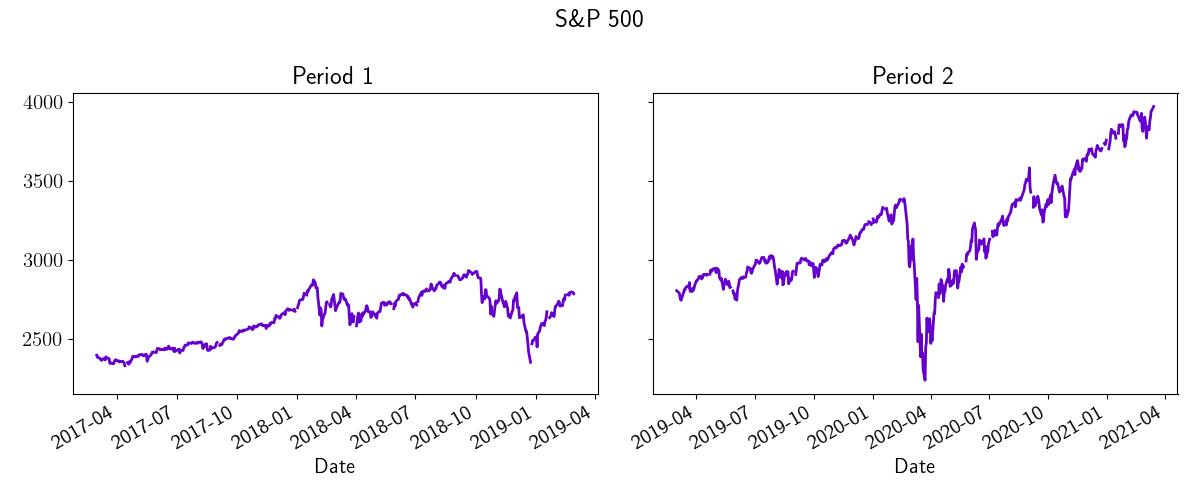
\includegraphics[width=15cm]{images/sp500.png}
    \caption{S\&P 500 of validation period}
    \label{fig:my_label}
\end{figure}




\subsection{System Parameter}
The threshold is the only adjusted parameter in the system.
We use three thresholds to represent different risk preferences.  
\begin{table}[htb]
    \centering
    \begin{tabular}{||c|c||}
    \hline \hline
    Threshold $\theta$ & Risk Preference \\ \hline
    No plenty ($\infty$) & High \\ \hline
    0.006 & Medium      \\ \hline
    0.002 & Low      \\ \hline \hline
    \end{tabular}
    \caption{Threshold and Risk Preferences}
    \label{tab:threshold}
\end{table}

\subsection{Baseline}
A Constant rebalanced portfolio (CRP) is an investment strategy that keeps a constant ratio between all investments over time. We use this to represent the portfolio provided by advisors to meet investors' risk preferences. We will use the average ratio of our portfolio to build a CRP portfolio and use it as a baseline for performance comparison in MDD and CAGR.
\subsection{Result}
Our system successfully delivers portfolios with different MDD to meet various investors' preferences, and output performed CRP in MDD and CAGR in most situations.

\begin{figure}[htb]
\centering
  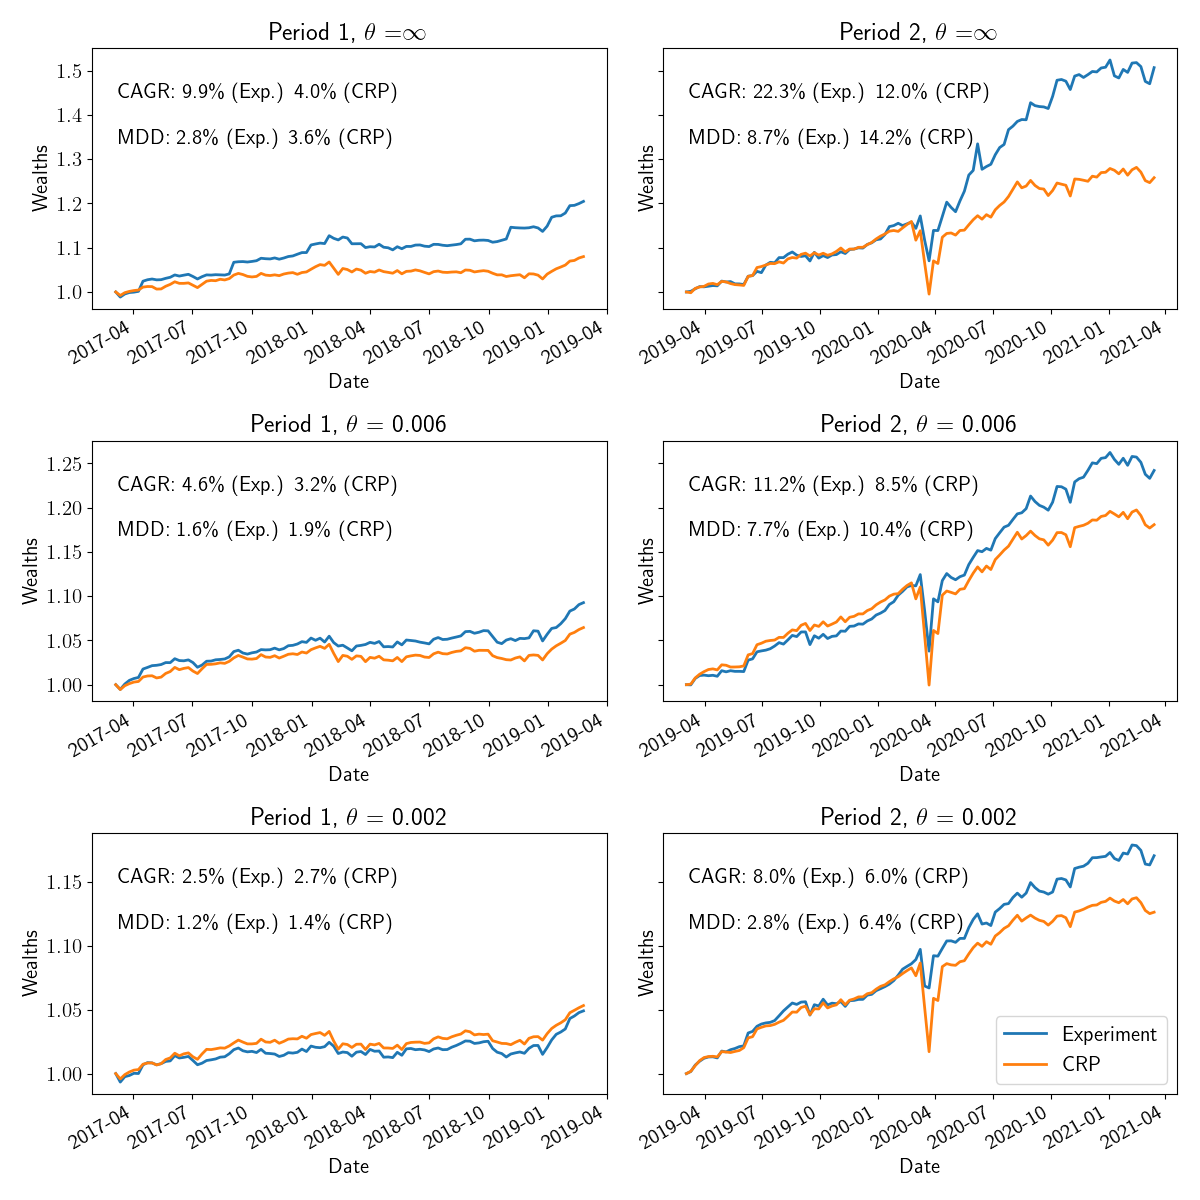
\includegraphics[width=16cm]{images/crp_compare.png}
  \caption [Comparison of experiments result with CRP]{Comparison of experiments result with CRP}
  \label{fig:crp_compare}
\end{figure}
% \chapter{Conclusions and Extensions}
\label{c:conclusion}
\secton{Conclusions}
\section{Extensions}

\appendix
\chapter{Selection of ETFs}
\label{appendix:etfs_corr}
\par
\begin{longtable}{|| m{2cm}| m{11.5cm}||}
\hline
Symbol & Name  \\ \hline \hline
SPY&SPDR S\&P 500 ETF \\ \hline
AGG&iShares Core U.S. Aggregate Bond ETF \\ \hline
BND&Vanguard Total Bond Market ETF \\ \hline
GLD&SPDR Gold Trust \\ \hline
LQD&iShares iBoxx \$ Investment Grade Corporate Bond ETF \\ \hline
BSV&Vanguard Short-Term Bond ETF \\ \hline
MBB&iShares MBS Bond ETF \\ \hline
IGSB&iShares Short-Term Corporate Bond ETF \\ \hline
SHY&iShares 1-3 Year Treasury Bond ETF \\ \hline
SHV&iShares Short Treasury Bond ETF \\ \hline

\end{longtable}
\chapter{Market Features}
\label{appendix:features_list}
\par
\begin{longtable}{|| m{10cm}| m{3.5cm}||}
\hline
Description & Categories \\ \hline \hline
5-Year Treasury Constant Maturity Rate & Interest Rates\\ \hline
10-Year Treasury Constant Maturity Rate & Interest Rates\\ \hline
30-Year Treasury Constant Maturity Rate & Interest Rates\\ \hline
5-Year Breakeven Inflation Rate & Interest Rates\\ \hline
10-Year Breakeven Inflation Rate & Interest Rates\\ \hline
Crude Oil Prices: Brent - Europe &  Commodities\\ \hline
Gold Prices &  Commodities\\ \hline
CBOE Volatility Index (VIX) &  Indexes\\ \hline
US Dollar Index (USDX) &  Currencies\\ \hline
\end{longtable}
\setlength\itemsep{-1em}

%
\chapter{Temp}

\section{Measure}
\(DD_T\)\cite{moody2001learning}
\[
DD_T = \sqrt{\cfrac{1}{T}\sum_{t=0}^{T}{min\{R_T,0\}^2}}
\]

VaR (Value at Risk)\cite{CoherentMeasuresofRisk}
\[
VaR_\alpha(X) = -inf \{x |P[X\leq x\cdot r]>\alpha \}
\]
Measure
RISK TOLERANCE FUNCTIONS\cite{elton2009modern}

\[f=\bar{R}-\frac{\tau^2}{T} \]
where T is referred to as risk tolerance and expresses the investor’s trade-off between
expected return and variance of return. 
\par
SAFETY FIRST\cite{elton2009modern}
If \(R_P\) is the return on the portfolio and \(R_L\) is the level below which the investor does not wish returns
to fall, Roy’s criterion is
\[Minimize P(R_p<R_L) \]
\section{Bitcoin}

\@startappendix


\backmatter

\clearpages
\phantomsection
\addcontentsline{toc}{chapter}{\bibname}
% Your bibliography goes here

\bibliography{
    bib/thesis-finance.bib,
    bib/thesis-ml.bib,
    bib/thesis-misc.bib
}


\end{document}
